\chapter{The Pi as a server, or something like that}


So far you've used your Pi and a lab machine individually, and hopefully have come to understand that they are both essentially the same kind of machine; they both run variations of the same operating system, and the principles you learn using one for the most part apply to the other. In the case of the Pi, you have complete control of the device as a super user, so can do what you like to it; in the case of the lab machines you have access to much more powerful hardware, but more restricted access to the filestore and operating system for reasons of security and privacy. 

Today, we will be getting your Pi and a desktop PC to communicate with one another, to reinforce the similarities between these setups, and to expose you to some of the principles of networking and remote access. 

\section{The LXDE window manager}

Connect your Pi up to the monitor, keyboard, mouse, network and power supply as before, and log in (remembering this time to use whatever password you set on the Pi rather than your University password, and the username `pi'). At the console, type

\begin{ttoutenv}
$ startx
\end{ttoutenv}

to start up X Windows and the Pi's default window manager, LXDE, which which appear moments later looking like the screenshot in Figure \ref{figure:lxde-desktop}. LXDE (the `Lightweight X11 Desktop Environment') is designed to be a lean, fast desktop environment, which makes it ideally suited for the Pi's modest CPU. Although rather less rich in features and `eyecandy' than Gnome, LXDE is a fully functioning environment that has all the features you will need for operating and programming the Pi. 

Down at the bottom of the screen you will see LXDE's `panel'. On the left of the panel (\protect\circled{1} in the figure) are controls that give you access to various applications, tools and system preferences. On the panel's right (marked \protect\circled{2}) are a CPU meter, a clock, a lockscreen control, and the logout button. On the desktop itself are shortcuts to some useful applications including a Terminal and Midori, which is a simple web browser. 

Spend a few minutes exploring the GUI. You'll almost certainly find that you're double-clicking on things that only need a single click, and vice versa, and may find that things aren't quite where you expect them to be---but rather than dismissing LXDE as being crude, embrace the differences; you may well find that you come to prefer its `no frills' approach to window managment over that of richer, heavier-weight environments such as Gnome. LXDE and other slimmed-down graphical environments consume considerably fewer CPU cycles and hence less power than their richer counterparts, and though this isn't an issue when you're running on a mains-powered desktop machine with a beefy graphics card such as the lab machines, this can be a serious issue devices running off batteries. 

\begin{figure}
\centerline{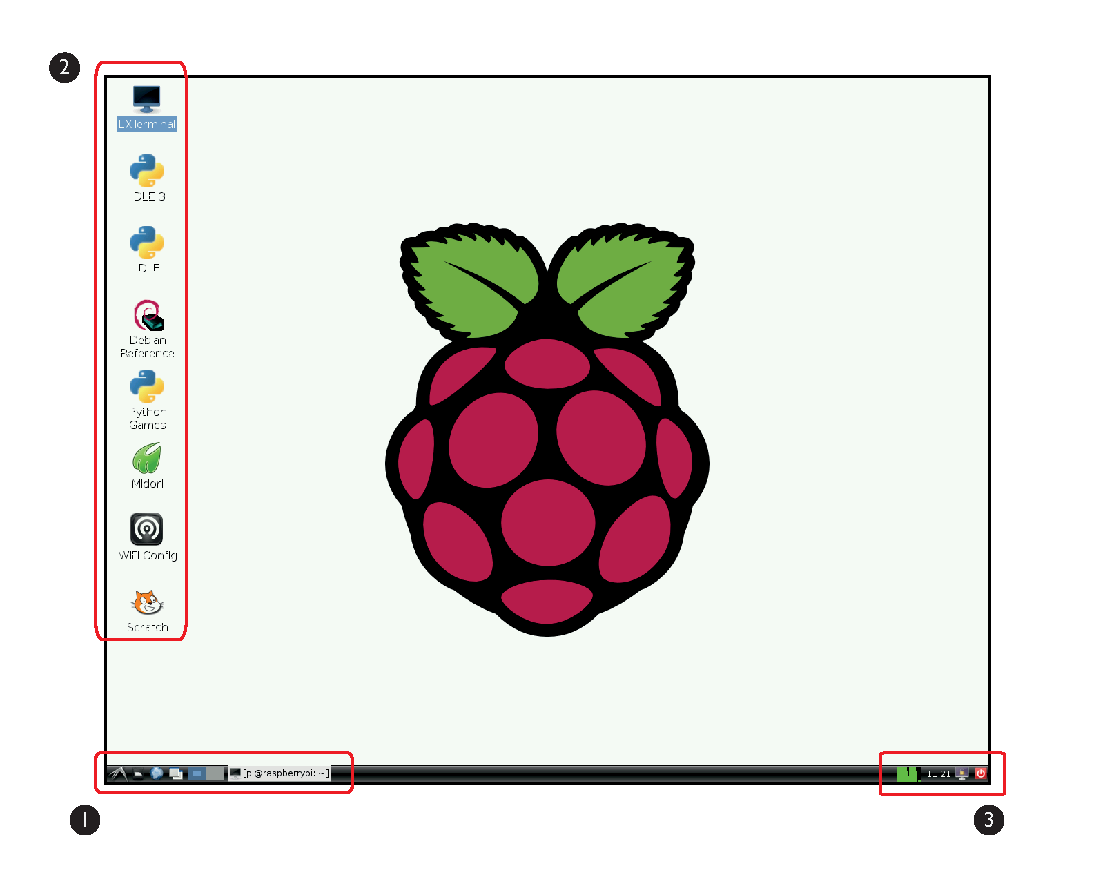
\includegraphics[width=14cm]{images/lxde-desktop}}
\caption{The Pi's default window manager is called LXDE.}\label{figure:lxde-desktop}
\end{figure}

\section{Configure mutt}

Once you've found your way around LXDE, fire up a Terminal so that we can configure your Pi to read your University email using Mutt. Unlike the lab machines, Mutt isn't installed by default on the Pi, so you'll need to do that yourself using

\begin{ttoutenv}
$ sudo apt-get install mutt
\end{ttoutenv}

Once the install has completed, we'll need to adjust Mutt's settings so that they once again point at your University email account. Now you could do this by following the instructions in the previous sessions's script again, but there's a much easier way: let's just copy the configuration file you created last time over on to the Pi. 

Let's confirm that we still have the \ttout{.muttrc} file that we'll need in our home filestore of our computer science account. We could unplug all the cables from the Pi, connect them back into the desktop PC and check that way, but that's no fun (especially because we'd then have to reverse it all to do the next bit of the exercise). So let's check remotely. 

Check out the hostname of the lab machine on your desk; it'll be written \ref{WHERE?}. In the terminal window on the Pi, issue a command like:

\begin{ttoutenv}
$ ssh USERNAME@HOSTNAME.cs.man.ac.uk
\end{ttoutenv}

obviously replacing USERNAME with your Univeristy username, and HOSTNAME with the name of the machine in front of you. You'll need to enter your university password, and should then be given a command prompt: notice that this command prompt no longer says \ttout{pi@raspberrypi}, but rather has the name of the machine you've just remotely logged into. The \ttout{ssh} command stands for `Secure Shell', and allows you to issue instructions to a remote machine as though you had logged in at that machine's console.

Type \ttout{ls -a} to confirm that your \fname{.muttrc} file is still where you expect it to be, and if all is well then press Ctrl+D to log out of the remote shell and get back to a shell running locally on your Pi (you'll see the command prompt change back to being `pi' again). Now we know the file is there, we want to copy it from your Computer Science filestore onto your Pi's local filestore.

To do this, we're going to use the \ttout{scp} (Secure Copy) command, which in some ways behaves like \ttout{cp}, but allows us to move files \textit{between} machines. 

Like \ttout{cp}, the \ttout{scp} command in its basic form takes two parameters, the first is the name of the source file (the one you want to copy, and the second is the name of the destination file (the one you want to create). The difference with \ttout{scp} is that either of these files can be on a remote machine, which means that you need to provide the command with enough information as to the location of the remote file in terms of the network and file system, and any login details necessary to get at it. The syntax of this is as follows:

\begin{ttoutenv}
username@hostname:filepath
\end{ttoutenv}

So for example, if you wanted to retrieve a file called \ttout{cheese.jpg} from the home directory of a user called \ttout{mrnoodle} that was stored machine with the host name \ttout{mypc.example.com}, and you wanted the local copy of the file to be called \ttout{mycheese.jpg} the command would be:

\begin{ttoutenv}
$ scp mrnoodle@mypc.example.com:cheese.jpg mycheese.jpg
\end{ttoutenv}

Then, supposing you had edited the file \ttout{mycheese.jpg} and wanted to put the file back into the home directory of the mrnoodle account but under a different name (so as not to over-write the original), you would issue:

\begin{ttoutenv}
$ scp mycheese.jpg mrnoodle@mypc.example.com:newcheese.jpg
\end{ttoutenv}

We're not exactly sure why MrNoodle and cheese feature quite so prominently in these exercises either, just go with the flow. Now use your new-found knowledge of \ttout{scp} to copy the \fname{.muttrc} file from your Computer Science account onto your Pi. Conveniently, there's nothing in the \fname{.muttrc} file that is specific to the Computer Science account setup, so you can use it as-is for Mutt on the Pi. Check that the file has copied over successfully using \ttout{less}, and then start up Mutt from a terminal. If everything has gone to plan, you should now be able to read and compose emails on your Pi. You can of course install other mail clients if you want to; there is a version of Thunderbird for the Pi called `icedove' (yes, yet another play on words!), or a much leaner graphical client called Claws Mail (which if you want to can be installed using \ttout{sudo apt-get install claws-mail}). Remember, though, that the memory card we've given you for your Pi is fairly small, so you probably don't want to clutter it up with uncecessary packages, and should find that Mutt is perfectly servicable for the occasional email. 

\section{X Windows again}

As we mentioned before, the X Windows system is a powerful beast, and although it was designed a long time ago (originating around 1984), was in many ways way ahead of its time.

Remember that the GUI you're now using on the Pi consists of two systems working together: X Windows (which amongst other things gives software access to the display hardware), and the Window Manager (in this case, LXDE) that provides the WIMP-style features such as movable windows and clickable controls. The X Windows system operates as a Client/Server architecture, where the `server' part does the drawing of stuff onto the screen, and clients request that things be drawn. One of the really nice features of X Windows is that it doesn't care too much about where the requests to draw things come from. Typically they come from processes that are running on the same hardware as the X Server, but this need not be the case as you're about to demonstrate.

Log back in to the lab PC using the \ttout{ssh} command, but this time include a \texttt{-X} switch before your username, something like:

\begin{ttoutenv}
$ ssh -X USERNAME@HOSTNAME.cs.man.ac.uk
\end{ttoutenv}

The \ttout{-X} switch tells the \ttout{ssh} program to redirect any X Windows requests back through the network from the remote machine to the X Server running on the local machine.

Confirm that you are indeed logged into your Computer Science account by checking the command prompt and using \ttout{ls} to make sure the files in your home directory are the ones you'd expect, and then type:

\begin{ttoutenv}
$ xeyes
\end{ttoutenv}

Googly eyes that follow the mouse! What's not to like? Well, okay, perhaps not hugely exciting in itself, but what's actually happening here is rather clever. The \ttout{xeyes} program is now running on the desktop machine; but the instructions to draw its graphical output are being forwarded over the secure shell connection you've made from the Pi to the lab machine, so that the Pi's X Windows system receives them. Press CTRL+C to abort \ttout{xeyes}, and instead try running \ttout{xterm}. You should see a new terminal window appear on your Pi's screen (which probably looks slightly different to the terminal you launch on the Pi a moment ago). This XTerminal, rather like xeyes, is actually running on the desktop machine---only its graphical representation is appearing on your Pi (if you use \texttt{ls} in that terminal, you'll see that its your Computer Science account that's visible, rather than your Pi's filestore). 

How could you use this feature to your advantage to give you a temporary graphical mail client (or perhaps to use Firefox as a web browser, rather than Midori) on the Pi, without needing to install any packages on the Pi itself?





create some simple html files with nano in a terminal window
run a simple python web server, and use midori to localhost to check all is lovely
quit graphical environment

At console
find the IP address of the Pi
disconnect keyboard / mouse /screen, back to desktop
interact with Pi via ssh
edit web pages, view them from desktop
install and configure apache

USB STICKS?

